\begin{figure}[h]  % h option suggests placing the figure here
	\centering  % Centers the figure
	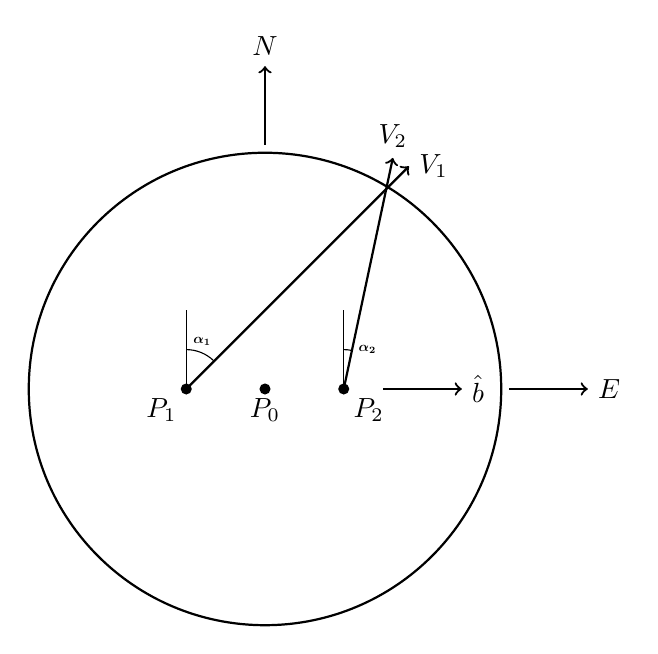
\begin{tikzpicture}
		% Define coordinates
		\coordinate (P0) at (0, 0);
		\coordinate (P1) at (-1,0);
		\coordinate (P2) at ( 1,0);
		
		% Draw circle
		\draw[thick] (P0) circle (3);
		
		% Draw P0ints
		\fill (P0) circle (2pt) node[below] {$P_0$};
		\fill (P1) circle (2pt) node[below left] {$P_1$};
		\fill (P2) circle (2pt) node[below right] {$P_2$};
		
		% Draw vectors
		\draw[->, thick] (0,3.1) -- ++(0, 1) node[above] {$N$};
		\draw[->, thick] (3.1,0) -- ++(1, 0) node[right] {$E$};
		
		% Direction vectors
		\draw[->, thick] (P1) -- ++({4*cos(45)}, {4*sin(45)}) node[right] {$V_1$};
		\draw[->, thick] (P2) -- ++({3*cos(78)}, {3*sin(78)}) node[above] {$V_2$};
		
		% Direction vector b-hat
		\draw[->, thick] (P2)+(0.5,0) -- ++(1.5, 0) node[right] {$\hat{b}$};
		
		% Angle alpha
	%		\draw[-] (P1) -- (P2);
	%		\draw[-] (P1) -- (P0);
	%		\draw[-] (P0) -- (P2);
		\draw (P1) -- ++(0,1);
		\draw (P2) -- ++(0,1);
		\draw (P1) ++(0.0,0.5) arc[start angle=90, end angle=45, radius=0.5];
		\draw (P2) ++(0.0,0.5) arc[start angle=90, end angle=78, radius=0.5];
		
		\node[scale=0.5, font=\boldmath] at (-.8,0.6) {$\alpha_1$};
		\node[scale=0.5, font=\boldmath] at (1.3,0.5) {$\alpha_2$};
		
		% Distance d_i
		%\draw[<->, thick] (P0) -- (P2) node[midway, right] {$d_i$};
	\end{tikzpicture}
    \caption{Intersection of two planes and a sphere.}
	\label{fig:CirclePlanePlane}  % Optional: Label for referencing
\end{figure}